\documentclass[utf8,14pt,a4paper,oneside,russian]{book}
\usepackage[14pt]{extsizes}
\usepackage{longtable}

%===========
%=Кодировка=
%===========
\usepackage[T2A]{fontenc}
\usepackage[utf8]{inputenc}
\usepackage[main=russian, english]{babel}

%===============
%=Римские цифры=
%===============
\newcommand{\RNumb}[1]{\uppercase\expandafter{\romannumeral #1\relax}}

%===================
%=Разметка страницы=
%===================
\usepackage[left=3cm, right=1cm, top=2cm, bottom=2cm, headheight=14pt, headsep=1cm, footskip=1cm]{geometry}
\pagestyle{plain}
\linespread{1.1} %Межстрочный интервад
\setlength{\parindent}{1.25cm} %Абзацный отступ
\setlength{\parskip}{0em} %Интервал между абзацами
\usepackage{indentfirst}

\usepackage{misccorr}
\usepackage{graphicx}
\usepackage{amsmath, amssymb, amsfonts}
\usepackage{xcolor} %пакет для работы с цветом
\usepackage{colortbl} %пакет для работы с цветом в таблицах

%===========
%=Заголовки=
%===========
\usepackage{titlesec}

\titleformat{\section}{\centering\large\bfseries}{\thesection.}{0.5em}{\MakeUppercase}
\renewcommand{\thesection}{\arabic{section}}
\renewcommand{\sectionmark}[1]{\markright{\thesection.~#1}}
\titlespacing*{\section}{0em}{2em}{1em}

\titleformat{\subsection}{\centering\normalsize\bfseries}{\thesubsection.}{0.5em}{}
\renewcommand{\thesubsection}{\arabic{section}.\arabic{subsection}}
\titlespacing*{\subsection}{0em}{1.25em}{0.5em}

\titlespacing*{\paragraph}{0em}{1.05em}{0.25em}

%=======
%=Языки=
%=======
\usepackage{algorithm} %пакеты для работы с алгоритмами
\usepackage{algpseudocode}

\usepackage{listings}

\usepackage{listings}
\lstdefinelanguage
{Assembler}
{morekeywords={CDQE,CQO,CMPSQ,CMPXCHG16B,JRCXZ,LODSQ,MOVSXD, %
		POPFQ,PUSHFQ,SCASQ,STOSQ,IRETQ,RDTSCP,SWAPGS, %
		rax,rdx,rcx,rbx,rsi,rdi,rsp,rbp, %
		r8,r8d,r8w,r8b,r9,r9d,r9w,r9b, %
		r10,r10d,r10w,r10b,r11,r11d,r11w,r11b, %
		r12,r12d,r12w,r12b,r13,r13d,r13w,r13b, %
		r14,r14d,r14w,r14b,r15,r15d,r15w,r15b, mov, times, bits, xor, int, cmp, dw, jmp, jz, inc, db}} % etc.

\lstloadlanguages{C, Python, Assembler, Java}

\definecolor{codegray}{rgb}{0.5,0.5,0.5}
\definecolor{gr}{rgb}{0.97, 0.97, 0.97}

\lstset{language=Assembler,
	extendedchars=true,
	belowcaptionskip=5pt,
	backgroundcolor=\color{gr},
	basicstyle=\ttfamily\normalsize,
	breakatwhitespace=false,         
	breaklines=true, 
	%escapechar=|,
	%frame=tb,
	numbers=left,                          
	numberstyle=\small\color{codegray},         
	stepnumber=1,                         
	numbersep=5pt,
	commentstyle=\itshape,
	stringstyle=\bfseries,
	keepspaces=true,
	showstringspaces=false,
	tabsize=2,
}

%============
%=Содержание=
%============
\usepackage{titletoc}
\makeatletter
\renewcommand{\tableofcontents}{\section*{Содержание}\markboth{Содержание}{}\@starttoc{toc}\newpage}
\makeatother
\titlecontents{section}[1.5em]{}{\contentslabel[\thecontentslabel.]{1.5em}}{}{\rule{0.1cm}{0pt}\titlerule*[0.75pc]{.}\contentspage}
\titlecontents{subsection}[4em]{\vspace{0.05em}}{\contentslabel[\thecontentslabel.]{2em}}{}{\rule{0.1cm}{0pt}\titlerule*[0.75pc]{.}\contentspage}

%========
%=Списки=
%========
\usepackage{enumitem}
\makeatletter
\AddEnumerateCounter{\asbuk}{\@asbuk}{м)}
\makeatother
\setlist{nolistsep, topsep=0.375em}
\setenumerate{leftmargin=2cm, labelsep=0em, labelwidth=0.75cm, align=left}
\setitemize{leftmargin=2cm, labelsep=0em, labelwidth=0.75cm, align=left}
\renewcommand{\labelitemi}{--}
\renewcommand{\labelenumi}{\arabic{enumi})}
\renewcommand{\labelenumii}{\asbuk{enumii})}
\renewcommand{\labelenumiii}{--}

%==========================
%=Математические операторы=
%==========================
\DeclareMathOperator{\mob}{Mob}
\DeclareMathOperator{\fix}{Fix}
\DeclareMathOperator{\ord}{ord}

\graphicspath{{pictures/}}
\DeclareGraphicsExtensions{.pdf,.png,.jpg}

\usepackage{tikz}
\usetikzlibrary{positioning}%for graph

\usepackage{neuralnetwork}

%гиперссылки
\usepackage[hidelinks]{hyperref}

%заглавные римские цифры
\newcommand{\RomanNumeralCaps}[1]
{\MakeUppercase{\romannumeral #1}}

\begin{document}
	
	\thispagestyle{empty}
	\small
	\begin{center}
		
\includegraphics[width=4.55cm]{logo_mirea}\\
		\MakeUppercase{Минобрнауки России}\\[1em]
		Федеральное государственное бюджетное образовательное учреждение\\
		высшего образования\\[0.5em]
		\textbf{<<МИРЭА -- Российский технологический университет>>}\\
		\textbf{РТУ МИРЭА}\\
		\rule{\textwidth}{0.75pt}\\
		Институт искусственного интеллекта\\
		Базовая кафедра №252 -- информационной безопасности\\[-0.45em]
		\rule{\textwidth}{0.75pt}\\[5em]
		\normalsize\MakeUppercase{\textbf{Курсовая работа}}\small\\[0.5em]
		По дисциплине\\ <<Математическая логика и теория алгоритмов>>\\[1.5em]
		Тема курсовой работы\\ \textbf{<<Сложные структуры данных и их использование для решения алгоритмических задач>>} \\[3em]
		\begin{tabular}{p{7cm}p{6cm}c}
			Студент группы ККСО-03-19 & Николенко В.О. & \rule{2cm}{0.75pt}\\[-0.5em]
			& & \footnotesize\textit{(подпись)}\small\\[1em]
			Руководитель курсовой работы &  & \rule{2cm}{0.75pt}\\[-0.5em]
			& & \footnotesize\textit{(подпись)}\small\\[5em]
			Работа представлена к защите & <<\rule{0.5cm}{0.75pt}>> \rule{2cm}{0.75pt} 2022 г. & \\[1em]
			Допущен к защите & <<\rule{0.5cm}{0.75pt}>> \rule{2cm}{0.75pt} 2022 г. & \\[1em]
		\end{tabular}
		\vfill
		Москва -- 2022
	\end{center}
	\normalsize
	\newpage
	
	% Содержание
	\tableofcontents
	
	% Первая глава
	\section{Введение}
	
	Алгоритмы - круто.
	
	\newpage
	\section{Сложные структуры данных}
	
	Простыми словами, \textbf{структура данных} - это контейнер, который хранит информацию в определенном виде. Из-за такой «компоновки» она может быть эффективной в одних операциях и неэффективной в других. Цель разработчика – выбрать из существующих структур оптимальный для конкретной задачи вариант.
	
	Данные являются самой важной сущностью в информатике, а структуры позволяют хранить их в организованной форме.
	
	Какую бы проблему ни решал инженер, ему приходится иметь дело с данными — будь то зарплата сотрудника, цены на акции, список покупок или даже простой телефонный справочник.
	
	В зависимости от ситуации данные должны храниться в некотором определенном формате. Структуры данных предлагают несколько вариантов таких размещений.
	
	Самые распространённые структуры данных:
	
	
	1. Массив (Array)
	
	2. Стек (Stack)
	
	3. Очередь (Queue)
	
	4. Связный список (Linked List)
	
	5. Дерево (Tree)
	
	6. Граф (Graph)
	
	7. Префиксное дерево (Trie)
	
	8. Куча
	
	9. Хэш-Таблица (Hash Table)
	
	В данной курсовой работе, мы рассмотрим структуры с 4 по 8 пункт включительно, так как все остальные незаурядны и  в дополнительном обзоре не нуждаются. Плюс к этим 5 способам хранения информации я бы хотел добавить передовые технологии: дерево хешей (дерево Меркла). Дерево хешей - технологии реализованные в блокчейне, так что их рассмотрение будет наиболее полезным для понимания его работы.
	
	\subsection{Связный список}
	
	Первая структура данных, которую мы рассмотрим - \textbf{связный список}. На то есть две причины:
	
	- связный список используется практически везде - от ОС до игр;
	
	- на его основе строится множество других структур данных (тот же HashMap при возникновении коллизий).
	
	Существует две версии связного списка: односвязный и двусвязный. Принципиальное отличие двусвязного от односвязного состоит в том, что во втором можно двигаться в двух направлениях, то есть узел (контейнер) указывает на последующий элемент и на предыдущий одновременно.
	
	\begin{center}
		\textbf{Односвязный список:}\\
		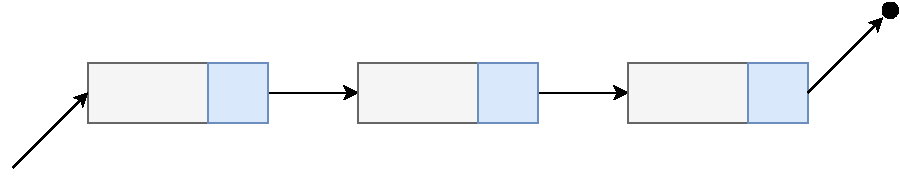
\includegraphics[scale=1]{linked_list_1}\\
		\textbf{Двусвязный список:}\\
		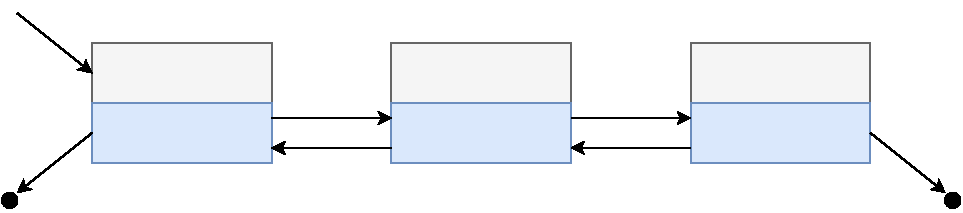
\includegraphics[scale=1]{linked_list_2}\\
	\end{center}
	
	Рассмотрим тогда сложность выполнения операций в связном списке:
	
	\begin{longtable}{c|c|c|c|c}
		Метод: &Добавление&Удаление элемента&Поиск&Удаление списка\\\hline
		Сложность: &O(n)&O(n)&O(n)&O(1)\\
	\end{longtable}

	$\bullet$ Операция добавления элемента в список - итерация до его конца (n эл-тов) и назначение указателя последнего элемента на новый контейнер.
	
	$\bullet$ Операция поиска элемента - итерация по списку до того как мы найдём эл-т, если натыкаемся на конец списка - return false.
	
	$\bullet$ Операция удаления элемента - выполнение операции поика и переназначение указателя предыдущего элемента на последующий контейнер, либо до конца списка (n эл-тов) и возвращаем false, т.к. элемент в списке отсутсвует.
	
	$\bullet$ Операция удаления списка - переназначение указателей \_head и \_tail в ноль.

	Можно дополнительно оптимизировать структуру и, допустим, хранить указатель на последний элемент, так мы сможем добиться ускорения добавления элемента в список до $O(1)$.
	
	Исходя из таблицы, с такой структурой работать над большими объёмами данных будет просто невозможно. Так что если она и используется, то только в особых случаях.
	
	\subsection{Деревья (бинарное, AVL, RB tree)}
	
	\textbf{Дерево} - одна из наиболее широко распространённых структур данных в информатике, эмулирующая древовидную структуру в виде набора связанных узлов. Является связным графом, не содержащим циклы. Большинство источников также добавляют условие на то, что рёбра графа не должны быть ориентированными.
	
	\subsubsection{Бинарное дерево}
	
	\textbf{Бинарное дерево} - это иерархическая структура данных, в которой каждый узел имеет значение (оно же является в данном случае и ключом) и ссылки на левого и правого потомка. Узел, находящийся на самом верхнем уровне (не являющийся чьим либо потомком) называется корнем. Узлы, не имеющие потомков (оба потомка которых равны NULL) называются листьями.
	
	Оно обладает дополнительными свойствами: значение левого потомка меньше значения родителя, а значение правого потомка больше значения родителя для каждого узла дерева. То есть, данные в бинарном дереве поиска хранятся в отсортированном виде.
	
	\begin{center}
		\textbf{Бинарное дерево:}\\
		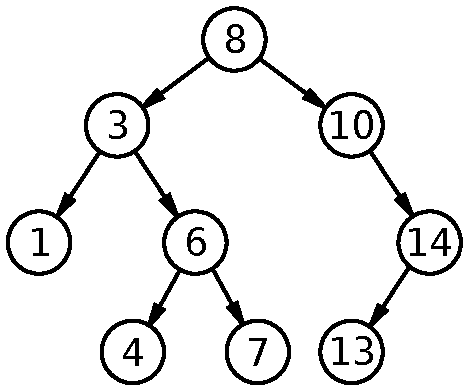
\includegraphics[scale=1]{binary_tree}\\
	\end{center}
	
	Рассмотрим тогда сложность выполнения операций в бинарном дереве:
	
	\begin{longtable}{c|c|c|c|c}
		Метод: &Добавление&Удаление эл-а&Поиск&Удаление дер-а\\\hline
		Сложность (ср.): &O(log n)&O(log n)&O(log n)&O(1)\\
		Сложность (худ.): &O(n)&O(n)&O(n)&\\
	\end{longtable}

	Сложность (худ.) здесь означает, что дерево будет перебрано полностью. Примером может служить экстремально несбалансированное дерево:
	
	\begin{center}
		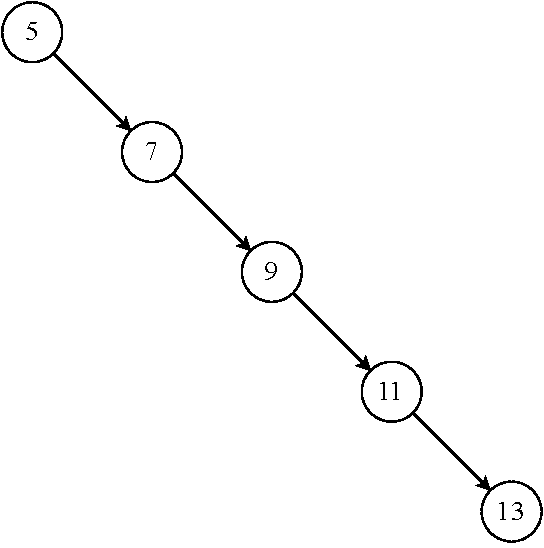
\includegraphics[scale=1]{unbalanced_bin_tree}\\
	\end{center}
	
	Это дерево тоже не очень нам подходит для работы с большими обёмами данных, хоть оно и даёт нам воможность осуществлять поиск / удаление / добавление за $O(log(n))$, но не гарантирует этого, худший вариант всё ещё имеет место быть.
	
	\subsubsection{AVL дерево}

	\textbf{AVL дерево} - самобалансирующееся бинарное дерево поиска. Тут исключён худший вариант, как в обычном бинарном дереве, т.к.  для любого узла дерева высота его правого поддерева отличается от высоты левого поддерева не более чем на единицу.
	
	\begin{center}
		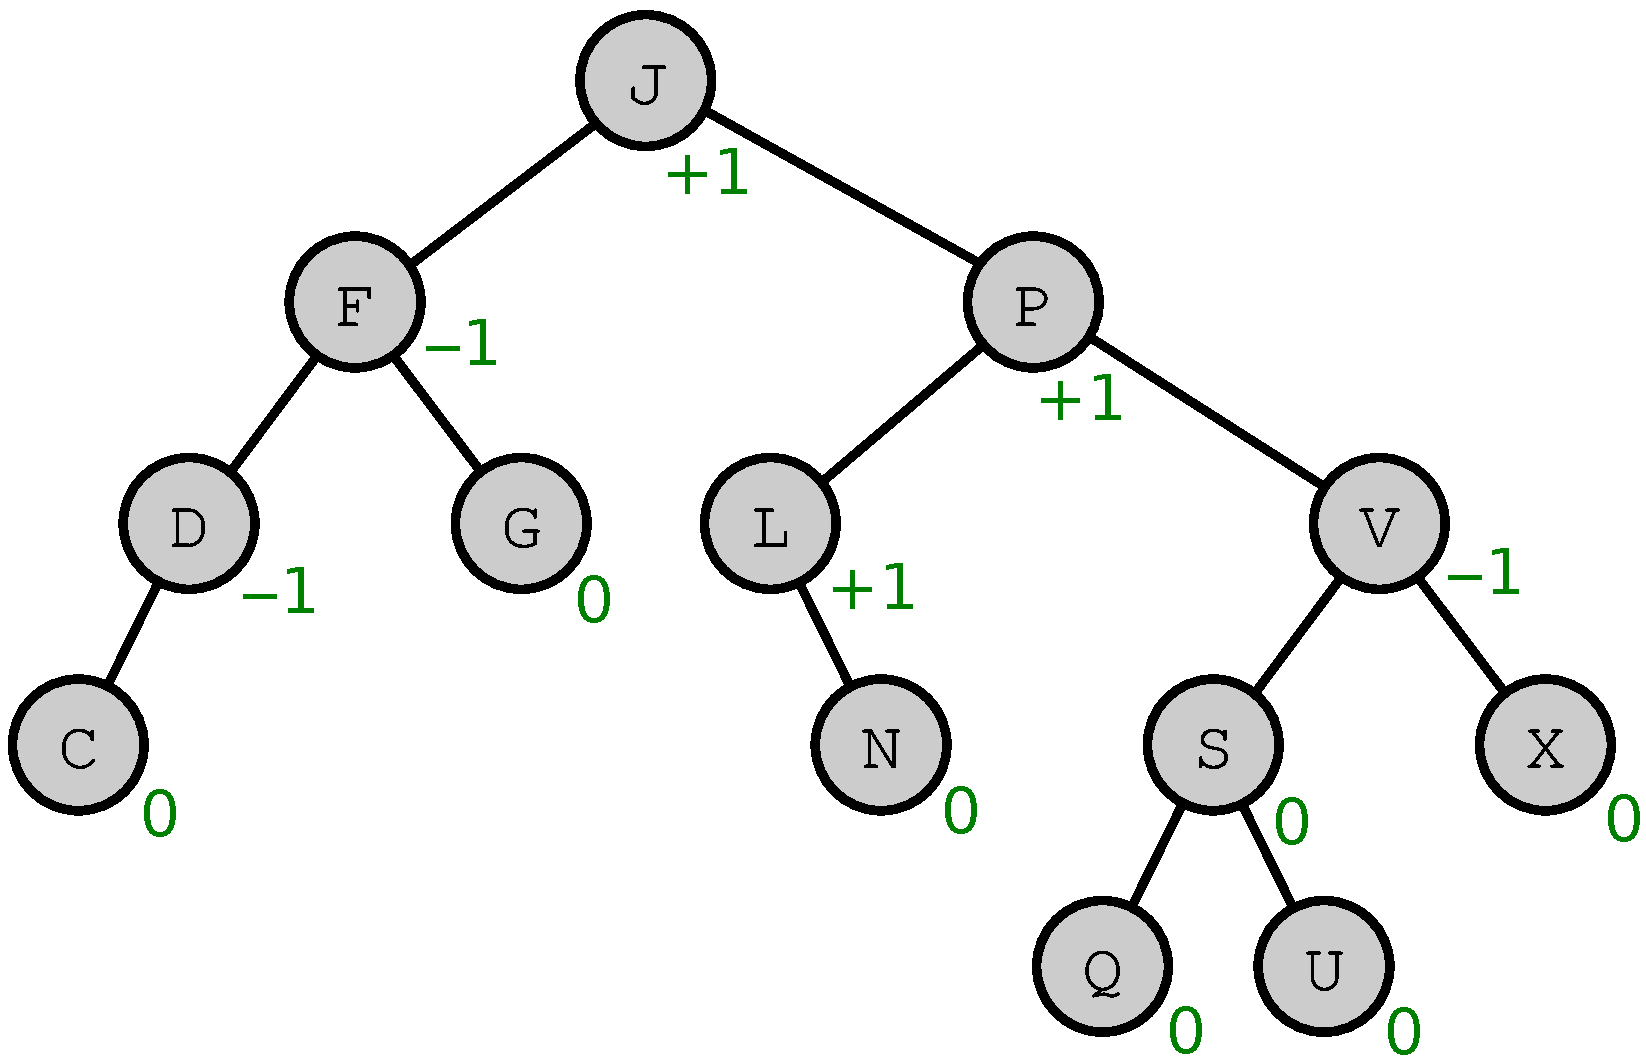
\includegraphics[scale=0.5]{avl_tree}\\
	\end{center}
	
	Из таблицы сложности операции уходит строка со сложностью в худшем варианте:
	
	\begin{longtable}{c|c|c|c|c}
		Метод: &Добавление&Удаление эл-а&Поиск&Удаление дер-а\\\hline
		Сложность (ср.): &O(log n)&O(log n)&O(log n)&O(1)\\
	\end{longtable}

	Однако, из-за сложности операций балансировки считается, что сбалансированные деревья
	следует использовать лишь в том случае, когда поиск информации происходит значительно
	чаще, чем добавление. 
	
	\subsubsection{RB tree}
	
	\textbf{Красно-Чёрное дерево (Red-Black tree)} - двоичное дерево поиска, в котором баланс осуществляется на основе "цвета" узла дерева, который принимает только два значения: "красный" (англ. red) и "чёрный" (англ. black). При этом все листья дерева являются фиктивными и не содержат данных, но относятся к дереву и являются чёрными. Для экономии памяти фиктивные листья можно сделать одним общим фиктивным листом.
	
	\begin{center}
		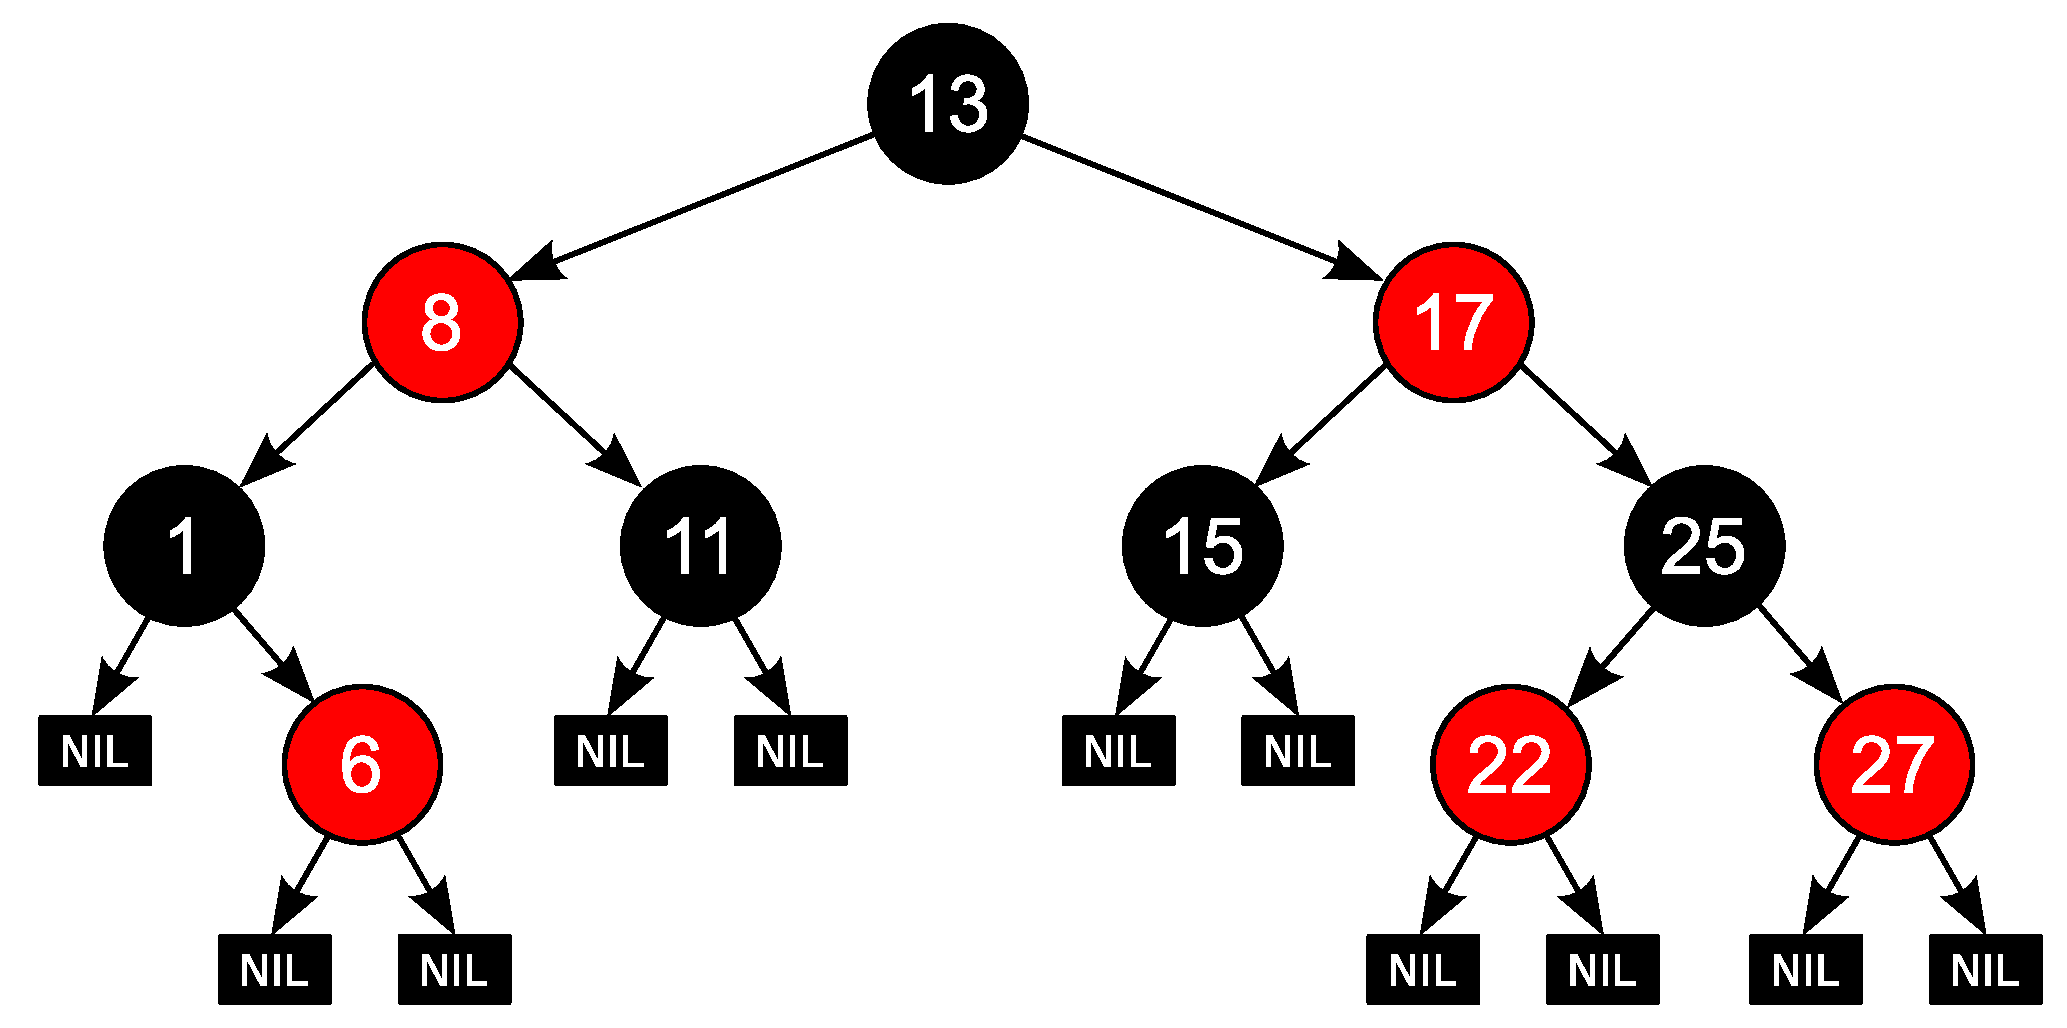
\includegraphics[scale=0.45]{rb_tree}\\
	\end{center}
	
	Красно-чёрным называется бинарное поисковое дерево, у которого каждому узлу сопоставлен дополнительный атрибут - цвет и для которого выполняются следующие свойства:
	
	$\bullet$ Каждый узел промаркирован красным или чёрным цветом
	
	$\bullet$ Корень и конечные узлы (листья) дерева — чёрные
	
	$\bullet$ У красного узла родительский узел — чёрный
	
	$\bullet$ Все простые пути из любого узла x до листьев содержат одинаковое количество чёрных узлов
	
	$\bullet$ Чёрный узел может иметь чёрного родителя
	
	Таблица временной сложности будет аналогична таблице для AVL дерева:
	
	\begin{longtable}{c|c|c|c|c}
		Метод: &Добавление&Удаление эл-а&Поиск&Удаление дер-а\\\hline
		Сложность (ср.): &O(log n)&O(log n)&O(log n)&O(1)\\
	\end{longtable}

	В данном случае, как и с AVL деревом, производительность для всех операций является оптимальной, чтоб уже использовать данную структуру как хранилище для объёмных данных.
	
	\subsection{Граф}
	
	Структура данных \textbf{графа} представляет собой набор узлов, которые имеют данные и связаны с другими узлами.
	
	Другими словами, граф - это структура данных (V, E), которая состоит из:
	
	- коллекции вершин V.
	
	- набора рёбер E, представленный в виде упорядоченных пар вершин (u, v).
	
	\begin{center}
		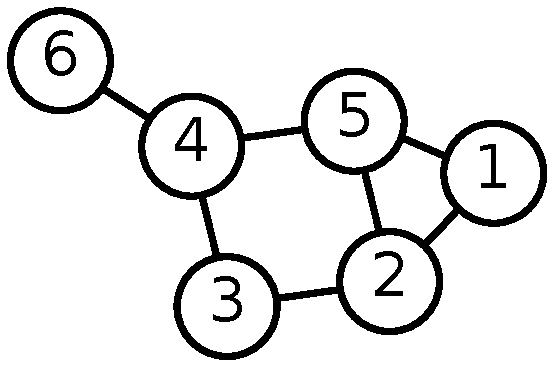
\includegraphics[scale=0.7]{graf}\\
	\end{center}
	
	Рассмотрим треминологию графа.
	
	Говорят, что вершина \textbf{смежна} с другой вершиной, если есть ребро, соединяющее их.
	
	Последовательность ребер, которая позволяет перейти от вершины A к вершине B, называется \textbf{путём}.
	
	Граф, в котором есть ребро (u, v) не обязательно означает, что также имеется ребро (v, u). Граф называется \textbf{ориентированным}, если его рёбра представлены стрелками, чтобы показать направление перехода.
	
	Наиболее распространенные операции над графами:
	
	- проверьте, присутствует ли элемент в графе;
	
	- обход графа;
	
	- добавить элементы (вершины, ребра) в граф;
	
	- нахождение пути от одной вершины к другой.
	
	Т.к. граф как структура данных используется редко и сама по себе является довольно экзотической, так что рассматривать сложность операций поиска, вставки и прочих не имеет смысла.
	 	
	\subsection{Префиксное дерево}
	
	\textbf{Префиксное дерево (иначе говоря нагруженное дерево или же trie)} - структура данных реализующая интерфейс ассоциативного массива, то есть позволяющая хранить пары «ключ-значение». Сразу следует оговорится, что в большинстве случаев ключами выступают строки, однако в качестве ключей можно использовать любые типы данных, представимые как последовательность байт (то есть вообще любые).
	
	Нагруженное дерево отличается от обычных n-арных деревьев тем, что в его узлах не хранятся ключи. Вместо них в узлах хранятся односимвольные метки, а ключем, который соответствует некоему узлу является путь от корня дерева до этого узла, а точнее строка составленная из меток узлов, повстречавшихся на этом пути. В таком случае корень дерева, очевидно, соответствует пустому ключу.
	
	\begin{center}
		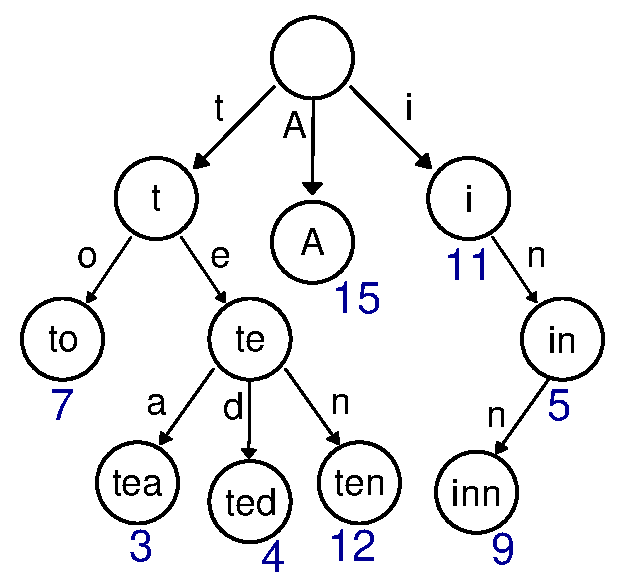
\includegraphics[scale=1]{trie}\\
	\end{center}
	
	Нагруженное дерево по показателям потребления памяти/процессорного времени не уступает хэш-таблицам и сбалансированным деревьям, а иногда и превосходит их по этим параметрам. Если обратить внимание на таблицу ниже, можно заметить, что в случае, когда $log(n)>|key|$, операции совершённые в префиксном дереве займут меньше времени, чем в том же AVL дереве.
	
	\begin{longtable}{c|c|c|c|c}
		Метод: &Добавление&Удаление эл-а&Поиск&Удаление дер-а\\\hline
		Сложность (ср.): &O(|Key|)&О(|Key|)&О(|Key|)&O(1)\\
	\end{longtable}

	По потреблению памяти нагруженное дерево часто выигрывает у хэш-таблиц и сбалансированных деревьев. Это связано с тем что у множества ключей в нагруженном дереве совпадают префиксы, и вместе с ними память которую они используют. Также, в отличии от сбалансированных деревьев, в нагруженном дереве нет необходимости хранить ключ в каждом узле.
	
	\subsection{Куча}
	
	\textbf{Куча} - полное бинарное дерево, для которого выполняется основное свойство кучи: приоритет каждой вершины больше приоритетов её потомков. В простейшем случае приоритет каждой вершины можно считать равным её значению. В таком случае структура называется max-heap, поскольку корень поддерева является максимумом из значений элементов поддерева.
	
	Дерево называется полным бинарным, если у каждой вершины есть не более двух потомков, а заполнение уровней вершин идет сверху вниз (в пределах одного уровня – слева направо).
	
	
	\begin{center}
		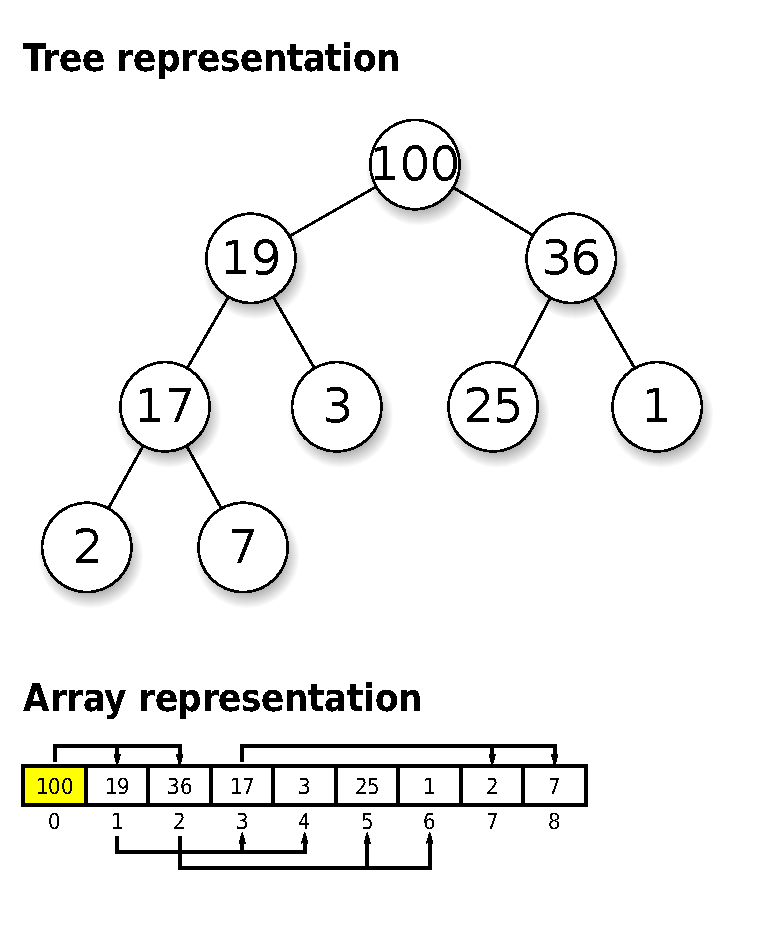
\includegraphics[scale=1]{heap}\\
	\end{center}
		
	Двоичную кучу удобно хранить в виде одномерного массива, причем левый потомок вершины с индексом i имеет индекс $2\cdot i+1$, а правый $2\cdot i+2$. Корень дерева - элемент с индексом 0. Высота двоичной кучи равна высоте дерева, то есть $log_2 N$, где $N$ - количество элементов массива.
	
	\begin{longtable}{c|c|c|c|c}
		Метод: &Добавление&Удаление эл-а&Поиск&Удаление дер-а\\\hline
		Сложность (ср.): &O(log n)&O(log n)&О(log n)&O(1)\\
	\end{longtable}
	
	\subsection{Хэш-Таблица}
	
	Хеш-таблица — это контейнер, который используют, если хотят быстро выполнять операции вставки/удаления/нахождения. 
	
	Любая операция внутри хеш-таблицы начинается с того, что ключ каким-то образом преобразуется в индекс обычного массива. Для получения индекса из ключа нужно выполнить два действия: найти хеш (хешировать ключ) и привести его к индексу (например, через остаток от деления).
	
	\begin{center}
		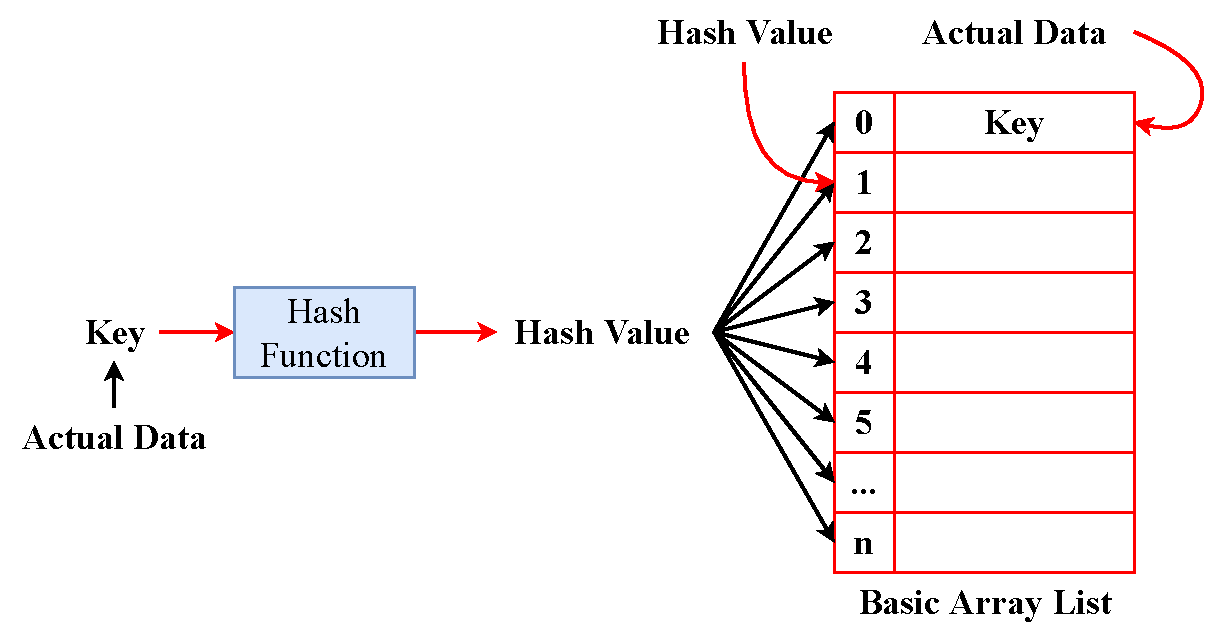
\includegraphics[scale=0.8]{hash_map}\\
	\end{center}
	
	Хеширование — операция, которая преобразует любые входные данные в строку (реже число) фиксированной длины. Функция, реализующая алгоритм преобразования, называется "хеш-функцией", а результат называют "хешем" или "хеш-суммой". Наиболее известны CRC32, MD5 и SHA (много разновидностей).
	
	\begin{longtable}{c|c|c|c|c}
		Метод: &Добавление&Удаление эл-а&Поиск&Удаление табл.\\\hline
		Сложность (ср.): &O(1)&O(1)&О(1)&O(1)\\
	\end{longtable}

	Однако, хэш-таблица очень требовательна к памяти. А так же существует слабое место - коллизии.
	
	Ключом в ассоциативном массиве может быть абсолютно любая строка (любой длины и содержания). Другими словами, множество всех возможных ключей — бесконечно. В свою очередь, результат работы хеш-функции — строка фиксированной длины, а значит множество всех выходных значений — конечно.
	
	Из этого факта следует, что не для всех входных данных найдётся уникальный хеш. На каком-то этапе возможно появление дублей (где под одним хешем лежит несколько разных значений — как если бы под одним индексом в массиве лежало два разных элемента). Такую ситуацию принято называть коллизией. Есть несколько способов разрешения коллизий (открытая адресация, метод цепочек), и каждому из них соответствует свой тип хеш-таблицы.
	
	\newpage
	\subsection{Дерево Меркла}
	
	Дерево Меркла - особый вид бинарного дерева, которое строится снизу вверх. А именно, пускай у нас имеется массив неких значений (не важно каких и в каком виде они представлены).
	
	Тогда на первом шаге мы применим функцию хэширования к каждому элементу по отдельности:
	
	
	\begin{center}
		$Hash_{00}=hash(L_1),$ $Hash_{01}=hash(L_2),\dots$\\
	\end{center}

	Так мы создали нижний уровень листов нашего дерева.
	
	На втором и последующих шагах, блоки, находящиеся уровнем выше, заполняются как хеши от суммы их детей:
	
	\begin{center}
		$Hash_{0}=Hash_{00}+Hash_{01},$ $Hash_{1}=Hash_{10}+Hash_{11}$\\
	\end{center}

	$+$ - конкатенация хэшей, обычно в ethereum для этого используется abi.encode ф-ия.
	
	Таким образом мы получаем верхушку дерева Меркла - Root Hash, который в последствии испольуется для проверки корректности данных введённых пользователем. В качестве хэш функции может использоваться как $keccak256$, так и $SHA256$.
	
	Хеш-деревья имеют преимущество перед хеш-цепочками или хеш-функциями. При использовании хеш-деревьев гораздо менее затратным является доказательство принадлежности определённого блока данных к множеству. Поскольку различными блоками часто являются независимые данные, такие как транзакции или части файлов, то нас интересует возможность проверить только один блок, не пересчитывая хеши для остальных узлов дерева.
	
	Пример работы дерва на практике:
	
	Пускай мы хоти доказать что транзакция, содержащаяся в $L_3$ - наша. Тогда мы должны предоставить сети некий proof, который будет массивом хешей: $[Hash_{11}, Hash_{0}]$. Тогда путём работы алгоритма полученный результат: 
	
	\begin{center}
		$Hash(Hash(Hash(L_3)+Hash_{11}) + Hash_{0})$\\
	\end{center}

	мы сверяем с root нашего исходного дерева, и в случае совпадения - мы доказали, что являемся владельцем этой транзакции и можем претендовать на какую-то монету, допустим.
	
	\begin{center}
		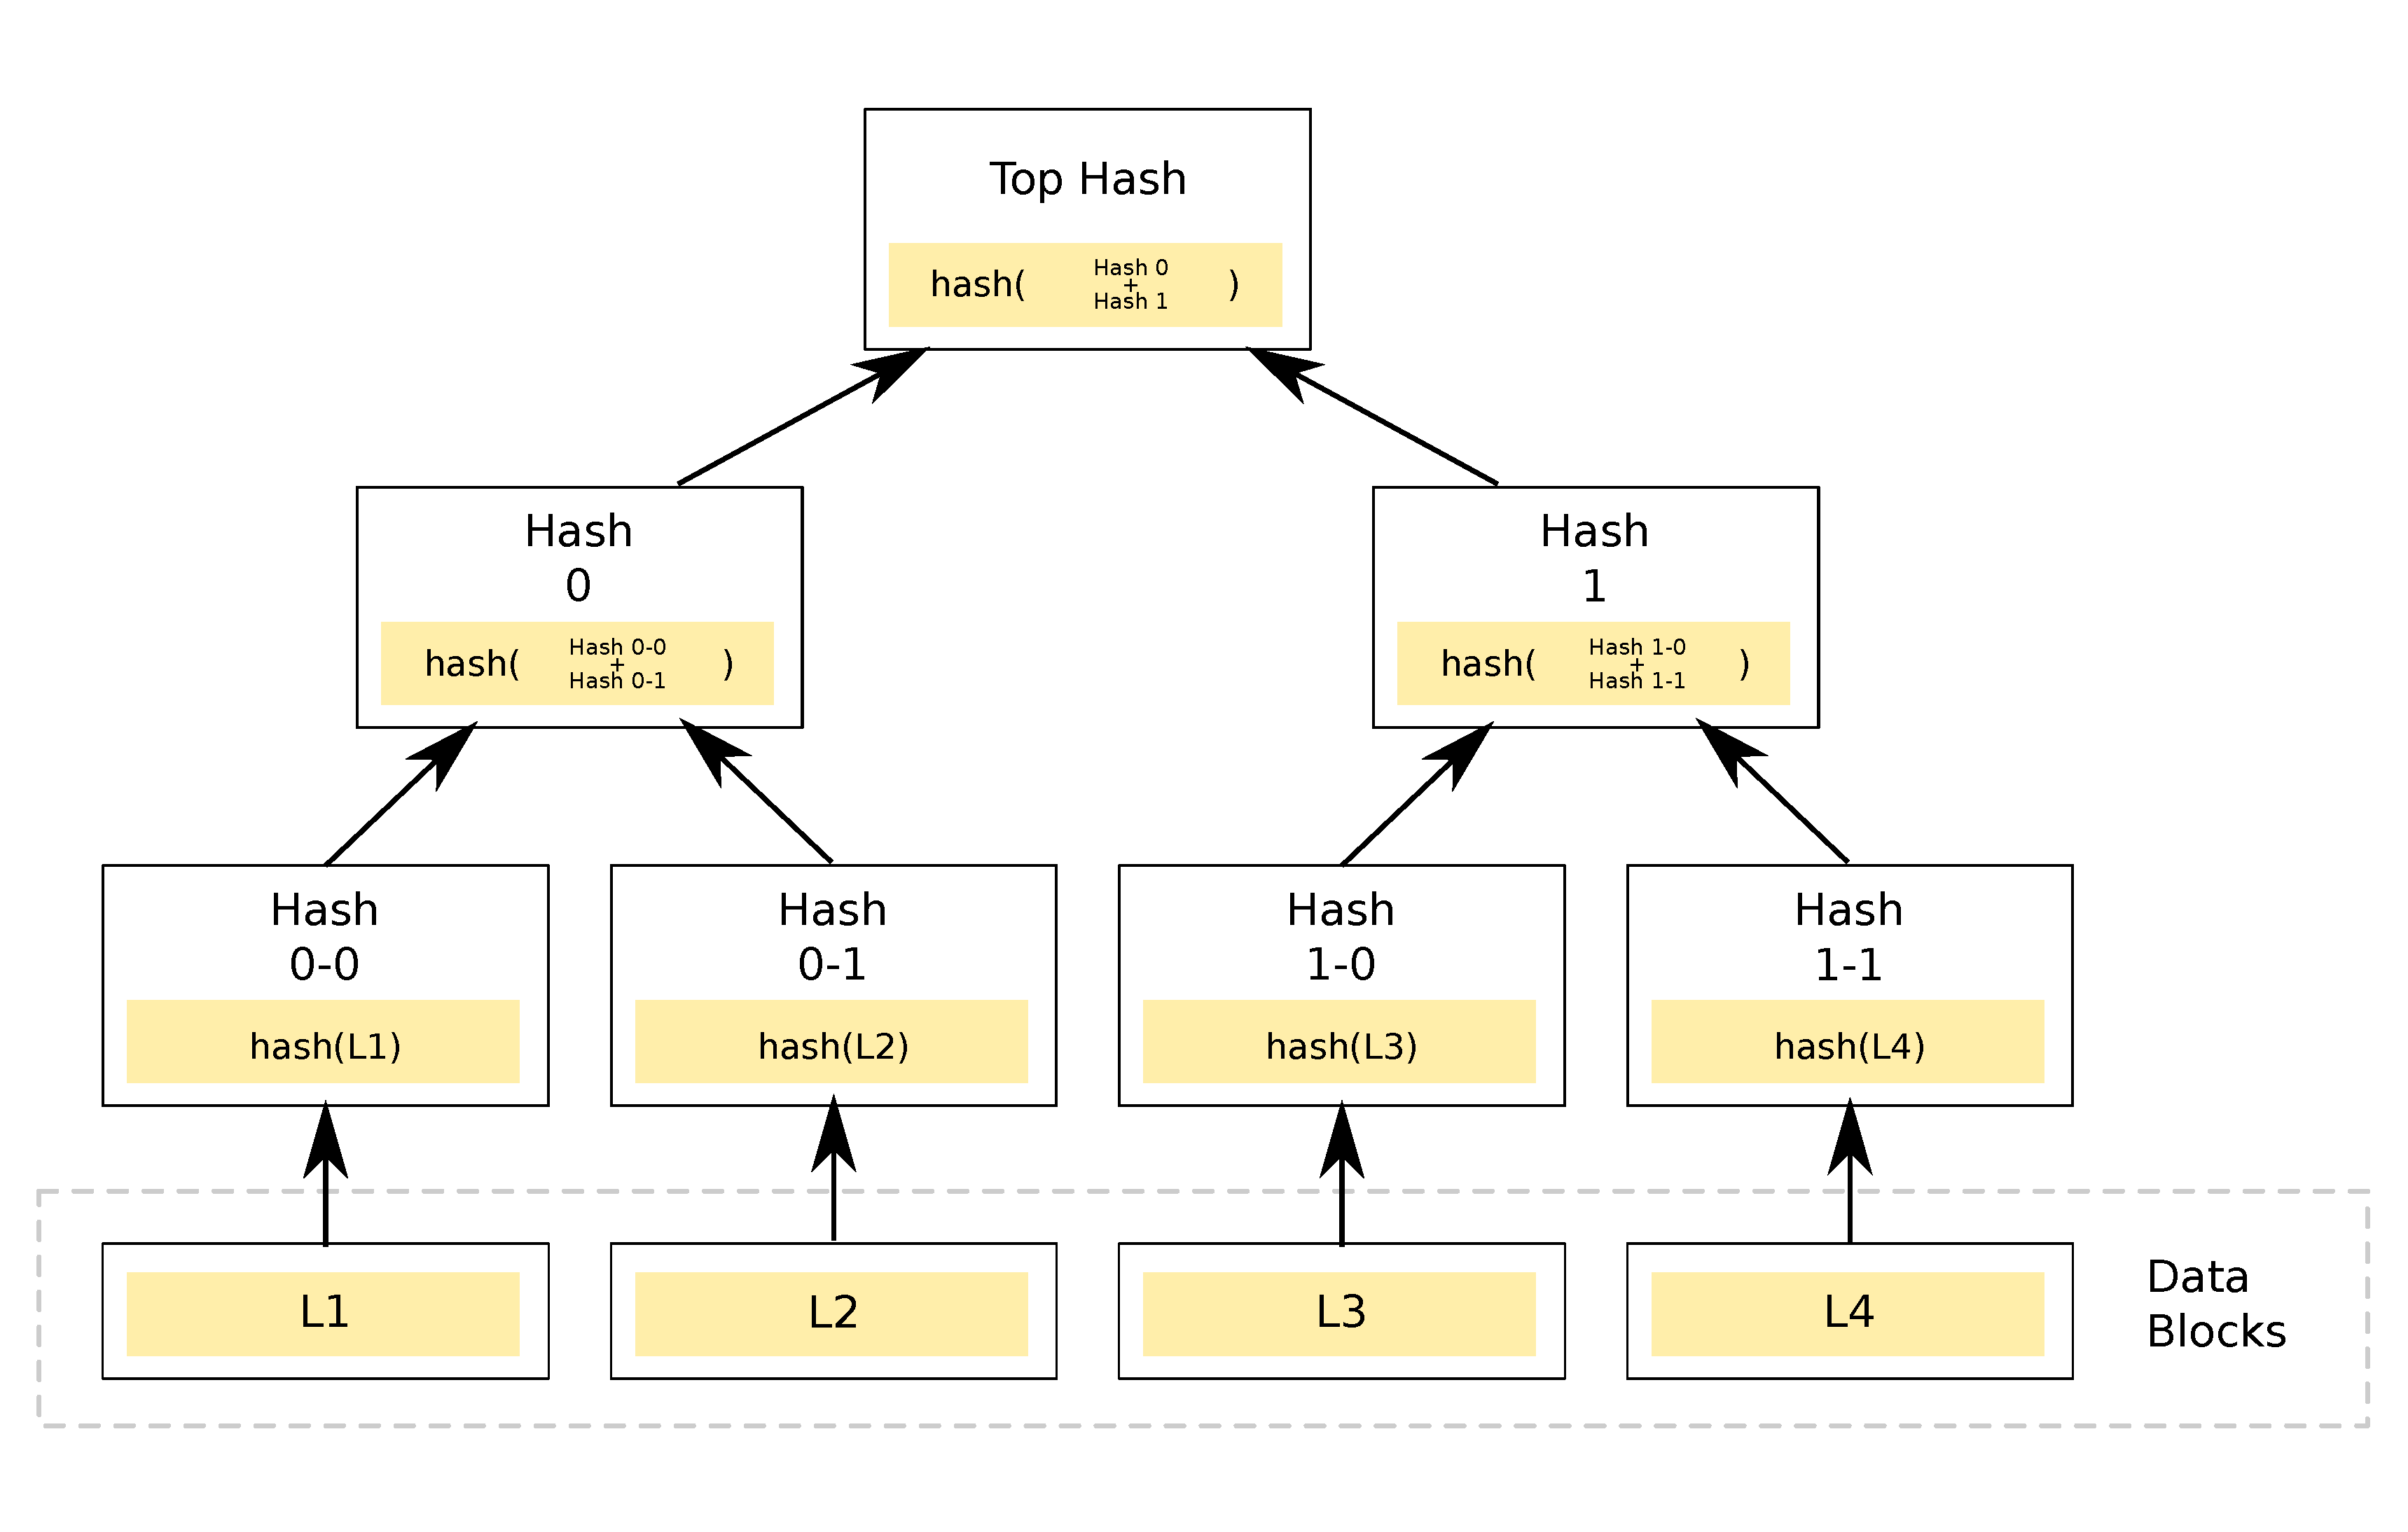
\includegraphics[scale=0.4, angle=-90]{hash_tree}\\
	\end{center}

	В общем случае можно записать формулу проверки так:
	
	\begin{center}
		$signature(L)=(L$ | $auth_{L_1},\dots,auth_{L_{K-1}})$,\\
		а проверку осуществить как $TopHash = Hash_K$\\
		$
		\left\{
		\begin{array}{ll}
			hash(L),&if$ $k=1\\
			hash(Hash_{k-1}+auth_{L_{k-1}}),&if$ $2\leq k\leq K\\
		\end{array}
		\right.
		$\\
	\end{center}

	\begin{longtable}{l|c|c|c|c}
		Количество транзакций&16&512&2048&65535\\\hline
		Приблизительный размер блока&4 кб&128 кб& 512 кб&16 мб\\\hline
		Размер пути (в хешах)&4&9&11&16\\\hline
		Размер пути (в байтах)&128&288&352&512\\
	\end{longtable}

	Таким образом, проверку можно выполнить за $O(K)=log_2N$, где $K$ - высота дерева.
	
	\newpage
	\section{Алгоритмы на структурах данных}
	
	Алгоритмы - круто! Ведь правда..?
	
	\subsection{Поиск высоты дерева}
	
	Одна из распространённых алгоритмических задачек - поиск минимальной и максимальной высоты дерева (допустим бинарного). Тут мы вспоминаем, что дерево, какое бы оно ни было, - тоже граф, так что к нему применимы алгоритмы на графах. В данном случае интересен поиск в ширину, который и поможет найти высоты дерева и выяснить, например, достаточно ли дерево сбалансировано.
	
	\textbf{Поиск в ширину, алгоритм:}
	
	1. Поместить узел $u$, с которого начинается поиск (в нашем случае корень дерева), в изначально пустую очередь.
	
	2. Извлечь из начала очереди узел $u$ и пометить его как посещённый и записать шаг на котором мы его посетили (расстояние от корня до узла).
	
	$\; \; \; \bullet$ Если узел $u$ является целевым узлом, то завершить поиск с результатом «успех».
	
	$\; \; \; \bullet$ В противном случае, в конец очереди добавляются все потомки узла $u$, которые ещё не были посещены и не находятся в очереди.
	
	3. Если очередь пуста, то все узлы связного графа были просмотрены, следовательно, целевой узел недостижим из начального; завершить поиск с результатом «неудача» (в случае с бинарным деревом такое недостижимо).
	
	4. Вернуться к пункту №2.
	
	\subsection{Поиск в глубину}
	
	Применяется:
	
	- В качестве подпрограммы в алгоритмах поиска одно- и двусвязных компонент;
	
	- В топологической сортировке;
	
	- Для поиска точек сочленения, мостов;
	
	- Для преобразования синтаксического дерева в строку (любую: префиксную, инфиксную, обратную польскую).
	
	\textbf{Алгоритм:}
	
	1. Пройдём по всем вершинам $v \in V$.
	
	$\; \; \; \bullet$ Если вершина $v$ белая, выполним для неё $DFS(v)$.
	
	Процедура DFS (параметр - вершина $u\in V$):
	
	1. Перекрашиваем вершину u u в серый цвет.
	
	2. Для всякой вершины $w$, смежной с вершиной $u$ и окрашенной в белый цвет, рекурсивно выполняем процедуру $DFS(w)$.
	
	3. Перекрашиваем вершину $u$ в чёрный цвет.
	
	Часто используют двухцветные метки — без серого, на 1-м шаге красят сразу в чёрный цвет. 
	
\end{document}